\documentclass[a4paper]{article}
\usepackage{float}
\usepackage[margin=1.2in]{geometry}
\usepackage[english]{babel}
\usepackage[utf8]{inputenc}
\usepackage{amsmath}
\usepackage{subcaption}
\usepackage{graphicx}
\usepackage{hyperref}
\usepackage{listings}
\usepackage[colorinlistoftodos]{todonotes}
\title{Student Discourse Through the Years}

\author{Benji Lu, Kai Fukutaki, Ziqi Xiong}

\date{\today}

\usepackage{Sweave}
\begin{document}
\maketitle

\Sconcordance{concordance:FinalProject.tex:FinalProject.Rnw:%
1 17 1 1 0 4 1 1 9 32 1 1 2 1 0 2 1 11 0 1 2 4 1 1 2 1 0 1 2 1 0 2 1 10 %
0 1 2 12 0 1 2 4 1 1 8 7 0 2 1 8 0 1 1 11 0 1 2 2 1 1 2 5 0 1 2 3 1 1 2 %
1 0 1 1 17 0 1 2 9 1 1 2 5 0 1 2 6 1 1 2 5 0 1 2 6 1 1 2 5 0 1 2 4 1 1 %
2 1 0 1 1 8 0 1 2 4 1 1 2 1 0 1 1 8 0 1 2 4 1 1 2 1 0 1 1 8 0 1 2 4 1 1 %
4 2 1 1 22 1 8 11 0 1 2 4 1 1 10 13 0 1 2 4 1 1 6 1 5 8 0 1 2 2 1 1 2 1 %
0 1 9 8 0 1 2 5 0 1 2 4 1 1 12 25 0 1 2 1 7 4 1 1 8 17 0 1 2 4 1 1 9 17 %
0 1 2 2 1 1 6 9 0 1 2 5 1 1 10 13 0 1 2 21 1}




\section{Motivation}
They say that those who do not know history are doomed to repeat it. We hope to show how campus dialogue on the Claremont Colleges has changed over time, using articles from The Student Life as representative of the discourse surrounding hot-button issues on campus. The Student Life, or TSL, is the oldest college newspaper in Southern California, and it is student-written and managed. It thus serves as a good glimpse into the thoughts and discourse of the students of the 5 Claremont Colleges (Pomona, Claremont McKenna, Scripps, Pitzer, Harvey Mudd). The student population itself is in a constant state of flux, as students generally spend only 4-5 years on campus. This ever changing population, and thus ever changing set of TSL writers (especially given that writers are probably working for TSL during their whole time on campus), means that issues in campus dialogue can repeatedly resurface when current students are not aware of the college discussions that took place four or five years ago. Plus, TSL does not have a `` static''  format; the number of articles published in each issue depends on the number of articles written, rather than publishing the same length paper each week. This allows for interesting data on word usage trends, topics covered, authorship, and more over time. How are topics evolving over time? Can we see major spikes in certain topics/phrases and trace those back to major events? Can we use these trends to inform our current dialogue? With better, more easily accessible information on TSL history, we can make it easier for future students to see what kind of discussion and action has taken place at the Claremont Colleges so that they can better understand the history of intellectual conversations on our campus and create fresher, deeper discussions in the future.

\section{Methodology}

\subsection{Data Source}

Our raw data was acquired directly from TSL's SQL database on ASPC peninsula server. The data is in the format of three csv tables: 

\begin{enumerate}
\item \textbf{articles}: This table contains the information related to the TSL articles, including id, title, content, status (published or not), created date, published date, updated date, section id and issue id.
\item \textbf{profiles}: This table contains the information related to the TSL staff, including id, name and position.
\item \textbf{articles\_profiles}: This table contains the authorship of TSL articles. Each row contains a TSL staff member id and an article id.
\end{enumerate}

We joined the three tables by article\_id and profile\_id and filtered out all the articles that are not published, do not have enough content (body text less than 50 words), or miss author or published date information. We selected important variables including title, content, published date, and author's name for our analysis.

To access the data we used, visit our code repository at \href{https://github.com/ZiqiXiong/TopicModeling}{https://github.com/ZiqiXiong/TopicModeling}.

\subsection{Model Training}

Our goal is to build an unsupervised model that cluster the TSL articles by their similarity in word usage so that each cluster can be labeled later and studied as a topic. With that goal in mind, we studied and used Latent Dirichlet Allocation(LDA) developed by Andrew Ng, et al., in 2003 for our project. LDA is a probabilistic model that allows sets of observations to be explained by unobserved groups that explain why some parts of the data are similar. When applied to a collection of text documents, LDA views each document as a mixture of a small number of topics and each word generated by one of the document's topics. With different inference techniques such as Gibbs Sampling, LDA is able to learn the composition of each topic (its associated word probabilities) and the topic mixture of each document.

Before training our LDA model, we first processed the body text of TSL articles by converting all words to lower case and reducing words to their stems, so that a group of words such as `` study'' ,`` Study''  and `` studies''  can be treated as one. We also removed punctuation, stop words (the most common, short function words), and extremely rare words that would only add noise to our model training. Finally, we transformed the collection of articles into a document-term matrix with each row representing an article and column representing a word. 

By using the R package `` topicmodel'', We trained multiple LDA models with different numbers of topics as input, including 25, 30, 35, 40, 45 and 50, so that we can use the most suitable model in our analysis later depending on how general we want the topics to be.

\subsection{Result and Visualization}

Our LDA model is capable of clustering key words into human-recognizable topic. Take five random topics discovered by our 40-topic model as an example:

\begin{Schunk}
\begin{Sinput}
> topic.terms = get.topic.terms(topic.model,20)
> set.seed(47)
> topic.terms[1:5,sample(40,5)]
\end{Sinput}
\begin{Soutput}
     Topic 40  Topic 15  Topic 29    Topic 31   Topic 21
[1,] "music"   "sex"     "student"   "student"  "game"  
[2,] "perform" "partner" "event"     "protest"  "fan"   
[3,] "song"    "feel"    "claremont" "black"    "player"
[4,] "band"    "sexual"  "communiti" "support"  "play"  
[5,] "play"    "make"    "colleg"    "movement" "season"
\end{Soutput}
\end{Schunk}

The 5 topics can be easily identified as ``music'', ``sex'', ``campus event'', ``student protest'', and ``sports game'' by their top keywords.

In addition to the distribution of words in topics, the LDA model can also calculates the percentage of a topic in an article and infers what the article is about. Take five random TSL articles for example:

\begin{Schunk}
\begin{Sinput}
> set.seed(37)
> # The primary topic of five articles
> sample.articles = articles[sample(5000,5),c(2,8)]
> names(sample.articles) = c('article.title','primary.topic')
> sample.articles
\end{Sinput}
\begin{Soutput}
                                              article.title primary.topic
2749 Women's Basketball Struggles Through Tough First Games             1
395       Peace, Popular Opinion, and the Prisoner Exchange            16
3243        Panel at CMC Debates Approach to Syria Conflict            10
2483                  Students Put Out Fire in Scripps Dorm            34
3592 Ye Olde TSL: 1927, The First Year of the Sponsor Group            27
\end{Soutput}
\begin{Sinput}
> # What the topics are about
> topic.terms[1:5, sample.articles[['primary.topic']]]
\end{Sinput}
\begin{Soutput}
     Topic 1   Topic 16 Topic 10  Topic 34  Topic 27 
[1,] "game"    "polit"  "student" "campus"  "student"
[2,] "sagehen" "state"  "discuss" "hall"    "pomona" 
[3,] "score"   "govern" "issu"    "student" "program"
[4,] "team"    "obama"  "chang"   "build"   "sponsor"
[5,] "sciac"   "presid" "talk"    "resid"   "colleg" 
\end{Soutput}
\end{Schunk}

As we can see from the result above, ``Women's Basketball Struggles Through Tough First Games'' is categorized into topic 1 about team sports, ``Peace, Popular Opinion, and the Prisoner Exchange'' into topic 16 about national politics, ``Panel at CMC Debates Approach to Syria Conflict'' into topic 10 about student discussion, `` Students Put Out Fire in Scripps Dorm'' into topic 34 about residential life, and ``Ye Olde TSL: 1927, The First Year of the Sponsor Group'' into topic 27 about Pomona sponsor program. 

Our model can also discover topics in articles that are not in our TSL dataset. For example, it can successfully categorize an 108-word excerpt from Martin Luther King's speech ``I Have a Dream'' into topic 16 about national politics and topic 31 about student protest.

\begin{Schunk}
\begin{Sinput}
> test.paragraph = "I have a dream that one day on the red hills of Georgia, 
+ the sons of former slaves and the sons of former slave owners will be able to sit down 
+ together at the table of brotherhood. I have a dream that one day even the state 
+ of Mississippi, a state sweltering with the heat of injustice, sweltering with the heat 
+ of oppression, will be transformed into an oasis of freedom and justice. I have a dream that 
+ my four little children will one day live in a nation where they will not be judged by the 
+ color of their skin but by the content of their character."
> test.result = classifyResult(test.paragraph,topic.model)
> test.result
\end{Sinput}
\begin{Soutput}
   Topic.ID    Weight
16       16 0.2469187
31       31 0.1954415
3         3 0.1920453
\end{Soutput}
\begin{Sinput}
> topic.terms[1:5, test.result[['Topic.ID']]]
\end{Sinput}
\begin{Soutput}
     Topic 16 Topic 31   Topic 3  
[1,] "polit"  "student"  "film"   
[2,] "state"  "protest"  "show"   
[3,] "govern" "black"    "charact"
[4,] "obama"  "support"  "movi"   
[5,] "presid" "movement" "play"   
\end{Soutput}
\end{Schunk}

After categorizing each article into its related topics, we are able to plot the frequency of a topic over time by counting the number of its articles every week. For example, here is the plot of topic 31 about student protest:

\begin{Schunk}
\begin{Sinput}
> topicgraph(articles,31,2,14)
\end{Sinput}
\end{Schunk}
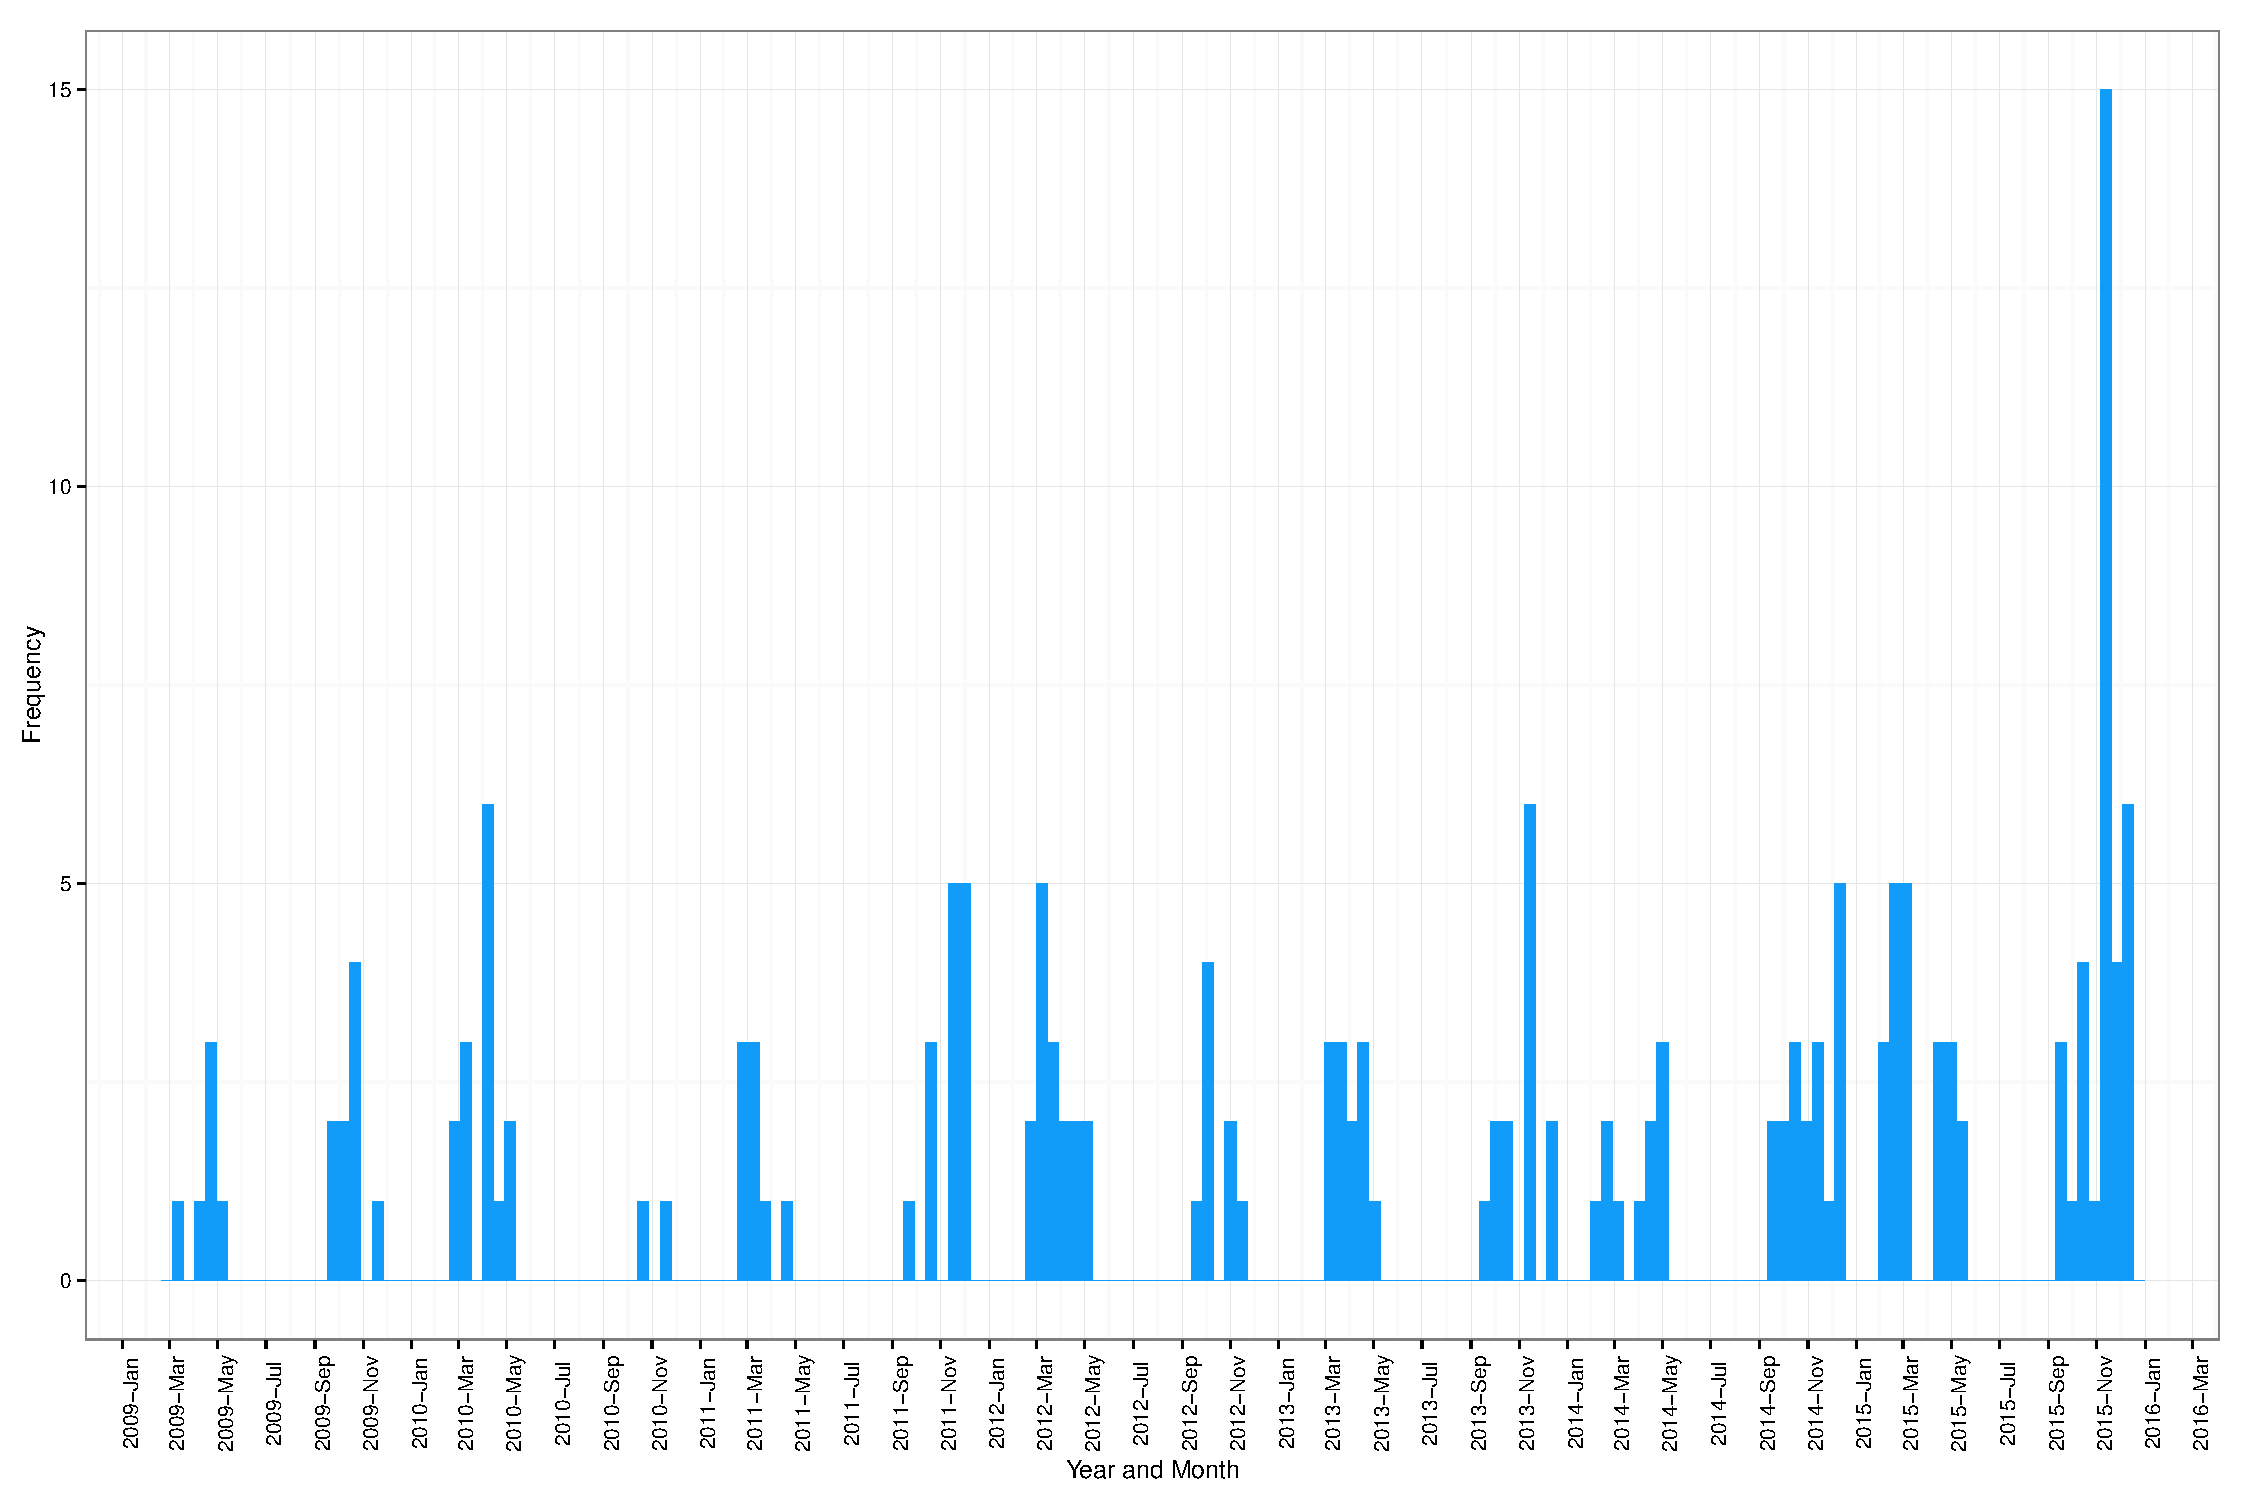
\includegraphics{FinalProject-005}

As we can see from the plot, the frequency of topic 31 experienced an unprecedented spike during the 2015 Fall semester, which reflects the heated discussion on the series of college protests in Yale, Mizzou and Claremont McKenna this fall.

We can also visualize what topics each author writes about. 

\begin{Schunk}
\begin{Sinput}
> print(authorChart(articles,'Editorial Board',2))
\end{Sinput}
\end{Schunk}
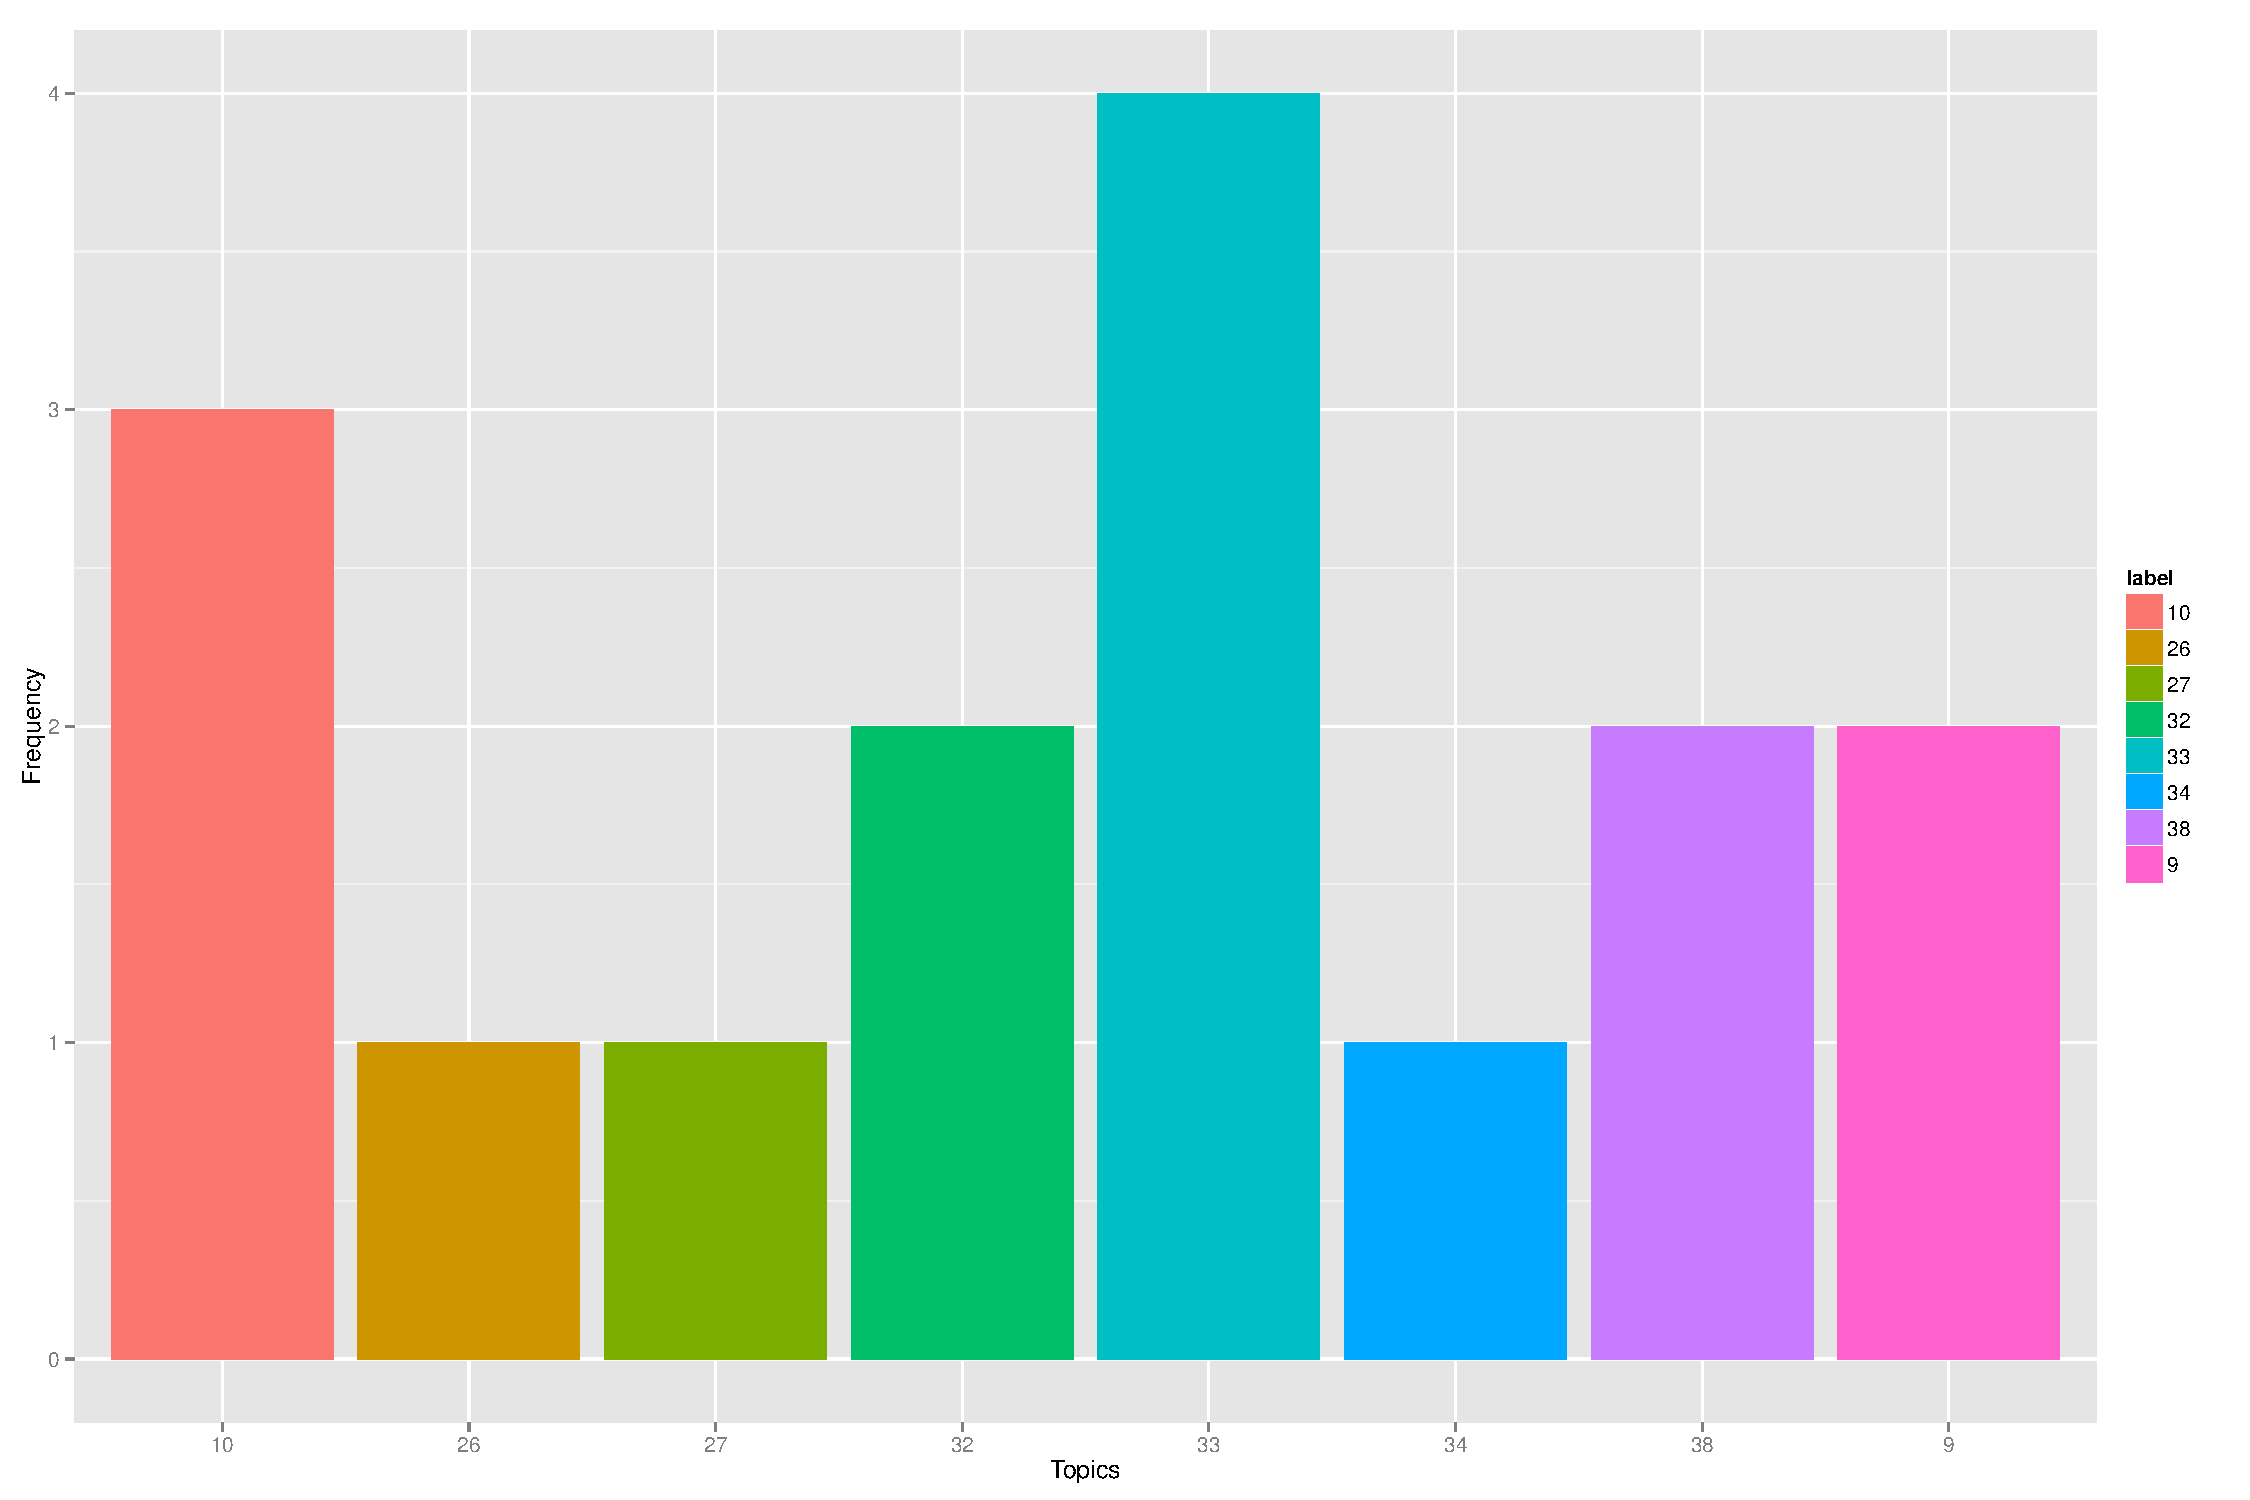
\includegraphics{FinalProject-006}


\section{Findings}

\subsection{Topic Analysis}

\subsection{Miscellaneous Insights}

\section{Conclusion}
Through topic analysis of the corpus of \textit{TSL} articles over the past five years, we were able to track how much coverage various subjects received in \textit{TSL} over time. From this, a rough idea of how these topics have been trending over time can be ascertained. For example, from our model we infer that [insert example].

However, our model faces several limitations, regarding both its analysis of topic coverage in \textit{TSL} and the inferences that can reasonably be drawn from its findings. Some of the topics generated through the model creation process are not very useful. For example, there are a few scattered `` Miscellaneous''  topics that have no logical continuity between the articles. The key words used for these miscellaneous topics have little relation to each other. This is due to [Kai: ZQ might need to go into more technical detail here about why the model will sometimes generate nonsensical topics]. For some numbers of topics, a topic based around weird punctuation or symbols that a few authors use is generated, since these are counted as distinctive words. Sometimes, topics are also combined, as is the case with `` Campus Activism''  combining both the divestment action and the action around the campus worker rights in 2012. [Benji: I can't speak as much to the limitations in Latent Dirichlet Allocation, so I'll talk about the inferences and someone else can fill in here.]

Latent Dirichlet Allocation is an unsupervised 

The model could also be improved to enable users to obtain a more accurate understanding of how the prominence of topics in campus discourse has changed over time. Perhaps most obviously, the frequency with which a \textit{TSL} article is visited online over a certain period of time likely is significant indicator of the prominence of the article's main topic during that period of time. Currently, the model does not include such information because the number of visitors was not tracked until this semester. As a result, certain topics are represented by the model as more prominent in campus discourse than perhaps they truly were. For example, our model produces three or four topics that are all essentially athletics. Moreover, since the sports section consistently covers sports events at the Claremont Colleges every issue of the newspaper, the model's visualization shows a consistently moderate number of \textit{TSL} articles covering sports, giving the impression that sports figure relatively prominently in the collective campus conscious. Without prior knowledge of our campus culture, it might be easy for someone to draw such an inference, when in fact athletics has a relatively modest place in campus dialogue. The frequency of visitors to each article would provide a different perspective: As shown in Section 4.2, sports articles generally had fewer online visitors than news and opinions articles this semester, and certain pieces related to race-based issues and Pomona branding received the most visitors. These data points are likely more consistent with the nature of campus discourse this past semester. If the model accounted for this type of information in its visualizations, it would present a more accurate picture of how topics trend over time.


\end{document}
